\section{Terahertz Wave Propagation in uniform nanorods}
\subsection{Introduction}
The dynamic testing of materials and components often involves predicting the propagation of stress waves in slender rods. The present work deals with the analysis of the wave propagation characteristics of nanorods. The nonlocal elasticity theory and also the lateral inertia are incorporated into classical/local rod model to capture unique features of the nanorods under the umbrella of continuum mechanics theory.
The strong effect of the nonlocal scale has been obtained which leads to substantially different wave behaviors of nanorods from those of macroscopic rods. Nonlocal rod/bar model is developed for nanorods including the lateral inertia effects. The analysis shows that the wave characteristics are highly overestimated by the classical rod model, which ignores the effect of small-length scale. The wave propagation properties of the nanorod obtained from the present formulations are compared with the continuum rod model, nonlocal second and fourth order strain gradient models, Born-Karman model and the nonlocal
stress gradient model. It has also been shown that, the unstable second order strain gradient model can be replaced by considering the inertia gradient terms in the formulations. The effects of both the nonlocal scale and the diameter of the nanorod on spectrum curves are studied.

\subsection{Nonlocal governing partial differential\\ equation for nanorods}
Figure \ref{nanorod} schematically describes a nanorod under discussion and
serves to introduce the axial coordinate x, lateral coordinate y, the
axial displacement $u = u(x,t)$the Young’s modulus $E$, the density $\rho$ the Poisson’s ratio $\nu$ and cross-sectional area $A$ . The displacement
field (X-direction), strain, strain rate and particle velocity associated with the displacement field in X-direction for this nanorod
are given by\\
\begin{equation}
u=u(x,t)
\end{equation}
\begin{equation}
\varepsilon_{xx}=\frac{\partial u}{\partial x}
\end{equation}
\begin{equation}
\dot{\varepsilon_{xx}}=\frac{\partial u}{\partial t} = \frac{\partial^2 u}{\partial x \partial t}
\end{equation}
\begin{equation}
V = \dot{u} = \frac{\partial u}{\partial t}
\end{equation}
\begin{figure}[b]
\centering
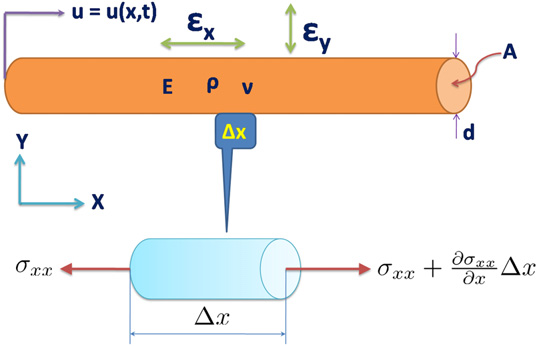
\includegraphics[scale=0.3]{nanorod}
\caption{A nanorod, showing Young’s modulus $E$, density $\rho$, Poisson’s ratio $\nu$, diameter $d$, cross-sectional area $A$, longitudinal displacement $u=u(x,t)$, strain along X-direction $\varepsilon_x$ and strains along Y-direction $\varepsilon_y$}
\label{nanorod}
\end{figure}
Due to Poisson’s ratio $\nu$, there are displacement fields $\nu$ and $w$ in
Y- and Z-directions, respectively. For example the strain and the
derivative of the displacement with time in the Y-direction are,
respectively,\\
\begin{equation}
\varepsilon_{yy}=-\nu \varepsilon_{xx}
\end{equation}
\begin{equation}
\dot{\nu}=-\nu y\dot{\varepsilon_{xx}}
\end{equation}
The kinetic energy of the infinitesimal length $\Delta$ of the rod (from Fig. \ref{nanorod}) is:\\
\begin{equation}
\Delta \Pi^e = \frac{1}{2} \rho A \Delta x (V^2+\nu^2 \xi^2 \dot{\varepsilon}^2_{xx})
\end{equation}
where $\rho$ is the density, $A$ is the cross-sectional area and $\xi$ is the
radius of gyration of the solid circular cross-section. Here, an
effective density is used to incorporate the effect of lateral inertia in
a one-dimensional nonlocal wave equation. An effective density $\rho_{eff}$ is now introduced such that the kinetic energy of the element $\Delta x$ is $\Delta \Pi^e_{eff}$, where\\
\begin{equation}
\Delta \Pi^e_{eff} =\frac{1}{2} \rho_{eff} A \Delta x V^2
\end{equation}
Using Newton’s second law, the net longitudinal force acting on the
element $\Delta x$ (see \ref{nanorod}) is:\\
\begin{equation}
\Delta \sigma_{xx} \times A = \rho_{eff} A \frac{\partial^2 u}{\partial t^2} \times x
\label{rhoeff}
\end{equation}
In the limiting case as $\Delta x \rightarrow 0$, equation \ref{rhoeff} becomes:\\
\begin{equation}
\frac{\partial \sigma_{xx}}{\partial x} = \rho_{eff} \frac{\partial^2 u}{\partial t^2}
\label{limcasesigma}
\end{equation}
To find the relationship between $\rho_{eff}$ and $\rho$, a functional $\cup_e$ is defined as the kinetic energy error when using the effective density, i.e.,\\
\begin{equation}
\bigcup_e = \iint [\Delta \Pi^e - \Delta \Pi^e_{eff} ] dx dt = 
\iint \left[ \dfrac{1}{2} \rho A (V^2 + \nu^2 \xi^2 \dot{\varepsilon}^2_{xx}) - 
\left( \dfrac{1}{2} \rho_{eff} A V^2 \right) \right] dx dt
\label{functionaldef}
\end{equation}
substituting for strain rate and particle velocity in \eqref{functionaldef} the
minimization of $\cup_e$ requires minimization of the following functional:\\
\begin{equation}
\bigcap_e = \iint \left\lbrace (\rho - \rho_{eff}) \left[\dfrac{\partial u}{\partial t}\right]^2 + \rho \nu^2 \xi^2 \left[ \dfrac{\partial^2 u}{\partial x \partial t} \right]^2 \right\rbrace dx dt
\end{equation}
The integrand of the functional $\cap_e$ is\\
\begin{equation}
f\left(\dfrac{\partial u}{\partial t},\dfrac{\partial^2 u}{\partial x \partial t}\right) = (\rho - \rho_{eff}) \left[\dfrac{\partial u}{\partial t}\right]^2 + \rho \nu^2 \xi^2 \left[ \dfrac{\partial^2 u}{\partial x \partial t}\right]^2
\label{func2}
\end{equation}
In order to minimize $\cap_e$ in Eq. \eqref{func2}, the integrand must satisfy the following equation:\\
\begin{equation}
\dfrac{\partial^2}{\partial x \partial t} 
\left[
 \dfrac{\partial f \left(\frac{\partial u}{\partial t},\frac{\partial^2 u}{\partial x \partial t}  \right)}{\partial \frac{\partial^2 u}{\partial x \partial t}}  
\right] 
- 
\dfrac{\partial}{\partial t}
\left[ 
\dfrac{\partial f \left(\frac{\partial u}{\partial t},\frac{\partial^2 u}{\partial x \partial t}  \right)}{\partial \frac{\partial u}{\partial t}}  
\right] = 0
\label{func3}
\end{equation}
Therefore, \eqref{func3} is identical to the following partial differential equation:\\
\begin{equation}
\rho_{eff} \frac{\partial^2 u}{\partial t^2} = \rho \frac{\partial^2 u}{\partial t^2} - \rho \nu^2 \xi^2 \frac{\partial^4 u}{\partial x^2 \partial t^2}
\label{effectivedenseq}
\end{equation}
The equation \eqref{effectivedenseq} gives the relationship between the effective density
S
and the density that minimizes the effective density error,$\cup_e$ defined in \eqref{functionaldef},over the length of the nanorod and the time of
motion. Substituting this expression in Eq. \eqref{limcasesigma} gives\\
\begin{equation}
\dfrac{\partial \sigma_{xx}}{\sigma x} = \rho \dfrac{\partial^2 u}{\partial t^2} - \rho \nu^2 \xi^2 \dfrac{\partial^4 u}{\partial x^2 \partial t^2}
\end{equation}
The constitutive model employed here is that obtained from the
theory of nonlocal/nonclassical continuum mechanics. For thin
rods Eq. \eqref{NLconsteqn} can be written in the following one dimensional form\\
\begin{equation}
\sigma_{xx} = \alpha^2 \frac{\partial^2 \sigma_{xx}}{\partial x^2} = E \varepsilon_{xx} = E \frac{\partial u}{\partial x}
\label{onedimconst}
\end{equation}
where $E$ is the modulus of elasticity,$\sigma_{xx}$ and $\varepsilon_{xx}$ are the local stress
and strain components in the $x$ direction, respectively, and $\alpha=e_0 a$ nonlocal scaling parameter. Differentiating the Eq. \eqref{onedimconst}with respect to $x$ on both sides, gives\\
\begin{equation}
\frac{\sigma_{xx}}{\partial x} - \alpha^2 \frac{\partial^3 \sigma_{xx}}{\partial x^3} = E \frac{\sigma_{xx}}{\partial x} = E \frac{\partial^2 u}{\partial x^2}
\label{diffonedimconst}
\end{equation}
Substituting equation \eqref{effectivedenseq} in eq. \eqref{diffonedimconst} gives\\
\begin{equation}
E \dfrac{\partial^2 u}{\partial x^2} = \rho \dfrac{\partial^2 u}{\partial t^2} - \rho \nu^2 \xi^2 \dfrac{\partial^4 u}{\partial x^2 \partial t^2} - \alpha^2 \rho \dfrac{\partial^4 u}{\partial x^2 \partial t^2} + \alpha^2 \rho \nu^2 \xi^2 \dfrac{\partial^6 u}{\partial x^4 \partial t^2}
\label{nonlocalinertia}
\end{equation}
Equation \eqref{nonlocalinertia} is the consistent fundamental governing equation of
motion for nonlocal rod model including the effect of lateral inertia/
Poisson’s effect. When $\alpha = e_0 a = 0\text{ and } \nu = 0$ , it is reduced to the equation of local or classical rod model.

\subsection*{Terahertz wave characteristics of nanorods}
For analyzing the ultrasonic/terahertz wave dispersion char-
acteristics in nanorods, we assume that a harmonic type of wave
solution for the displacement field u(x,t) and it can be expressed in
complex form as \cite{gopalakrishnan2008spectral,doyle1989wave}\\
\begin{equation}
u(x,t) = \sum_{p=0}^{P-1} \sum_{q=0}^{Q-1}\hat{u}(x,\omega_q)e^{-(k_p x - \omega_q t)}
\label{harmonicsoln}
\end{equation}
where $P$ and $Q$ are the number of time sampling points and number
of spatial sampling points, respectively, and $j=\sqrt{-1}$. $\omega_q$ is the
circular frequency at the $q$th time sample. Similarly, $k_p$ is the axial
wavenumber at the $p$th spatial sample point. Substituting Eq. \eqref{harmonicsoln} into the governing partial differential equation (eq. \eqref{nonlocalinertia}) we get
the characteristic equation (dispersion relation). The dispersion
relation is solved for the wavenumbers or wave frequencies. The
wave frequency is a function of wavenumber $k$, the nonlocal scaling
parameter $\alpha = e_0 a$and the material properties ($E, \nu,\text{ and } \rho$ of the
nanorod. This shows a non-linear relation between wavenumber
and wave frequency i.e., the obtained axial waves in nanorod are
dispersive in nature. The present results are compared with
the results obtained from classical continuum model, second and fourth order strain gradient models, stress gradient model and Born-K\'arm\'an model. If $\alpha = 0$ and $\nu = 0$ the wavenumber is directly
proportional to wave frequency, which will give a non-dispersive
wave behaviour (explained in \cite{doyle1989wave})

\subsection{Numerical results and discussion}
For the present analysis, a single-walled carbon nanotube is
assumed as a nanorod. The values of the radius, thickness, Young’s
modulus and density are assumed as 3.5 nm, 0.35 nm, 1.03 TPa,
and 2300 $\mathrm{kg/m^3}$ , respectively.
The present results are compared with the results obtained from
the following models:\\
\begin{itemize}
\item \textit{Classical/Local continuum model}:
	\begin{itemize}
	\item Constitutive relation:\\
		\begin{equation}
		\sigma(x) = E \varepsilon(x)
		\end{equation}
	\item Governing differential equation:\\
		\begin{equation}
			\dfrac{\partial^2 u(x,t)}{\partial x^2} = \dfrac{\rho}{E} 					\dfrac{\partial^2 u(x,t)}{\partial t^2}
		\end{equation}
	\item Dispersion relation:\\
		\begin{equation}
			k^2 + \dfrac{\rho}{E} \omega^2 = 0
		\end{equation}
	\end{itemize}
\item \textit{Nonlocal second order strain gradient model}:\\
	\begin{itemize}
	\item Constitutive equation:\\
	\begin{equation}
		\sigma(x) = E \left[ \varepsilon(x) + \alpha^2 \dfrac{\partial^2 \varepsilon(x)}		{\partial x^2} \right]
	\end{equation}
	\item Governing differential equation:\\
	\begin{equation}
	\alpha^2 \dfrac{\partial^4 u(x,t)}{\partial x^4} + \dfrac{\partial^2 u(x,t)}{\partial x^2} = \dfrac{\rho}{E} \dfrac{\partial^2 u(x,t)}{\partial t^2}
	\end{equation}
	\item Dispersion Relation:\\
	\begin{equation}
	\alpha^2 k^4 - k^2 + \frac{\rho}{E} \omega^2 = 0
	\end{equation}
	\end{itemize}
\item \textit{Nonlocal fourth order strain gradient model}:\\
	\begin{itemize}
	\item Constitutive equation:\\
	\begin{equation}
		\sigma(x) = E \left( \varepsilon(x) + \alpha^2 \dfrac{\partial^2 \varepsilon(x)}{\partial x^2}+ \alpha^4 \dfrac{\partial^4 \varepsilon(x)}{\partial x^4} \right]
	\end{equation}
	\item Governing differential equation:\\
	\begin{equation}
	\alpha^4 \dfrac{\partial^6 u(x,t)}{\partial x^6} + \alpha^2 \dfrac{\partial^4 u(x,t)}{\partial x^4} + \dfrac{\partial^2 u(x,t)}{\partial x^2} = \dfrac{\rho}{E} \dfrac{\partial^2 u(x,t)}{\partial t^2}
	\end{equation}
	\item Dispersion Relation:\\
	\begin{equation}
	-\alpha^4 k^6 + \alpha^2 k^4 - k^2 + \frac{\rho}{E} \omega^2 = 0
	\end{equation}
	\end{itemize}
\item \textit{Nonlocal stress gradient model}:\\
	\begin{itemize}
	\item Constitutive equation:\\
	\begin{equation}
		\sigma(x) - \alpha^2 \dfrac{\partial^2 \sigma(x)}{\partial x^2} = E \varepsilon(x)
	\end{equation}
	\item Governing differential equation:\\
	\begin{equation}
	\dfrac{\partial^2 u(x,t)}{\partial x^2} + \dfrac{\rho}{E} \dfrac{\partial^4 u(x,t)}{\partial x^2 \partial t^2} = \dfrac{\rho}{E} \dfrac{\partial^2 u(x,t)}{\partial t^2}
	\end{equation}
	\item Dispersion Relation:\\
	\begin{equation}
	-k^2 + \frac{\rho}{E}\alpha^2 \omega^2 k^2 +\frac{\rho}{E}\omega^2 = 0
	\end{equation}
	\end{itemize}
\item \textit{Born-K\'arm\'an model}:\\
	\begin{itemize}
	\item Dispersion Relation:\\
	\begin{equation}
	\omega = \frac{2}{a}\sqrt{\frac{E}{\rho}} sin\left(\frac{k\times a}{2}\right)
	\end{equation}
	\end{itemize}
\item \textit{Non-local stress gradient model (including lateral inertia)}:
	\begin{itemize}
	\item Fundamental governing equation:\\
	\begin{equation}
E \frac{\partial^2 u}{\partial x^2} = \rho \frac{\partial^2 u}{\partial t^2} - \rho \nu^2 \xi^2 \frac{\partial^4 u}{\partial x^2 \partial t^2} - \alpha^2 \rho \frac{\partial^4 u}{\partial x^2 \partial t^2} + \alpha^2 \rho \nu^2 \xi^2 \frac{\partial^6 u}{\partial x^4 \partial t^2}	
	\end{equation}
	\item Dispersion relation:\\
	\begin{equation}
	\omega = \sqrt{\dfrac{E}{\rho}} \dfrac{k}{\sqrt{(1+k^2 \alpha^2)(1+k^2 \xi^2 \nu^2)}}
	\end{equation}
	\end{itemize}
\end{itemize}

Fig. \ref{terahertz_freqresp} shows the variation of axial wavenumber of a nanorod with wave frequency. From Fig.\ref{terahertz_freqresp}, for a nanorod, it can be seen that there is only one mode of wave propagation i.e., axial or longitudinal. For local
or classical model, the wavenumbers for the axial mode has a linear
variation with the frequency which is in the tera-hertz (THz) range.
The linear variation of the wavenumbers denote that the waves will
propagate non-dispersively, i.e, the waves do not change their shapes
as they propagate. On the other hand, the wavenumbers obtained
from strain gradient/nonlocal stress gradient models have a non-
linear variation with the frequency, which indicates that the waves
are dispersive in nature. However, the wavenumbers of this wave
mode have a substantial real part starting from the zero frequency.
This implies that the mode starts propagating at any excitation
frequency and does not have a cut-off frequency (refer Fig \ref{terahertz_freqresp}).

\begin{figure}
\centering
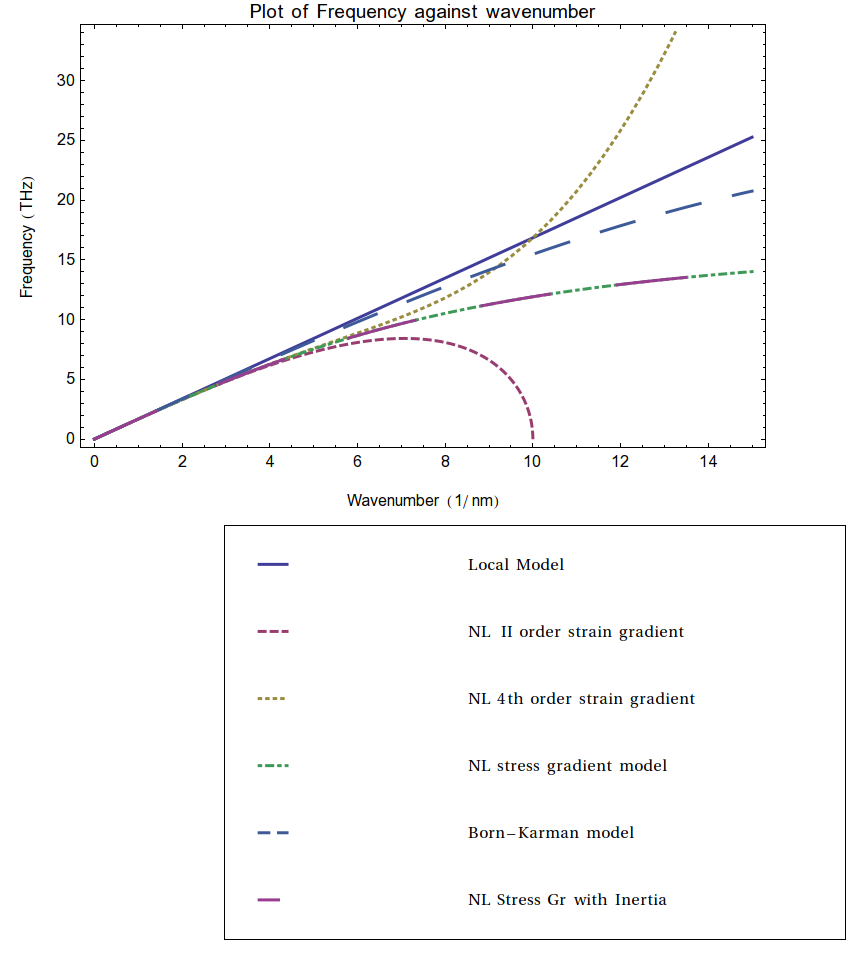
\includegraphics[scale=0.5]{terahertz_freq}
\caption{A Comparison of the wavenumber dispersion with wave frequency in a
nanorod obtained from classical/local and nonlocal theories suggested in literature
with the present result, to show the effect of lateral inertia.}
\label{terahertz_freqresp}
\end{figure}

The spectrum curves for nanorod obtained from both second
and fourth order strain gradient models are also shown in Fig. \ref{terahertz_freqresp}, for
comparison. As said, the spectrum relations obtained from the
classical continuum model shows that the waves in nanorod are
non-dispersive. But both the strain gradient models shows that the
waves in nanorod are dispersive in nature. It can also be seen that
the fourth order strain gradient model give improved approxima-
tion over the second order strain gradient model, as compared to
the classical continuum model (such observations are also made
in \cite{narendar2010ultrasonic}). The results are compared with the Born-K\'arm\'an model, as well as the nonlocal stress gradient model. This result shows an improved approximation over the second
order strain gradient model (see Fig. \ref{terahertz_freqresp}).It can be concluded that, the
instability of the second order strain gradient model can be
overcome by considering the inertia gradients.
The cut-off value for the wave number, i.e., the
wave number for which the angular frequency is zero, dominates
the static response of the second order strain gradient model. This cut-off emerges at $k=1/\sqrt{\alpha}$ (see Fig. \ref{terahertz_freqresp}). While for the fourth-
gradient model it only concerns the higher wave numbers, see
Fig. \ref{terahertz_freqresp}. However, in the response of the fourth order strain gradient model the effect of these high frequency waves are of minor
importance. Due to the nonuniqueness and instability of the second
order strain gradient model will give quite different wave behavior
compare to the fourth order strain gradient model. The unstable
second order strain gradient model can made stable by considering
the inertia gradients in the formulation.

The effect of the scaling parameter on the wave dispersion
relation in nanorod is shown in Fig. \ref{varyalpha}. As the nonlocal scaling
parameter $(\alpha = e_0 a)$ increases, the frequency of the wave will
decrease with an increase in the wavenumber. Here $\alpha$ values are
assumed from 0.0 to 1.0 nm. As $\alpha$ tends to larger value, the wave
frequency becomes very smaller at higher values of wavenumber as
shown in Fig. \ref{varyalpha}. It can be seen that, while dealing with the nonlocal
elasticity theory including the effect of lateral inertia, on should not
neglect the scaling parameter. So, the scaling parameter plays an
important role while dealing with the dynamics of nanostructures.

\begin{figure}
\centering
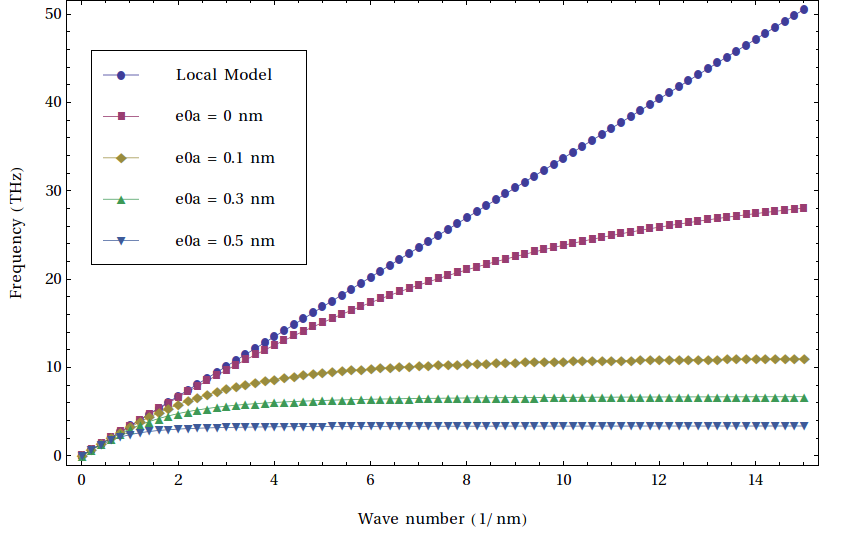
\includegraphics[scale=0.5]{tera_alphavary.png}
\caption{Wavenumber dispersion (including the effect of lateral inertia) with wave
frequency in a nanorod for various values of the nonlocal scaling parameter $\alpha$}
\label{varyalpha}
\end{figure}

The effect of radius of nanorod, on the wave dispersion relation
based on the present formulation is shown in Fig. \ref{varyradius}. For the present
analysis, we considered three different radii of nanorods i.e., 1.0,
2.0 and 5.0 nm. For comparison, the results obtained from local/
classical elasticity are also shown in the figure. As the radius of the
nanorod increases, the wave frequency becomes almost constant for
wavenumbers larger than 5.0 $\text{nm}^{-1}$. The effect of the lateral inertia
shows that, as the radius of the nanorod increases, the wavenumber
decreases and will not become constant irrespective of the wavenumber. The instability of the second order strain gradient
model can be overcome by considering the inertia gradients.

\begin{figure}
\centering
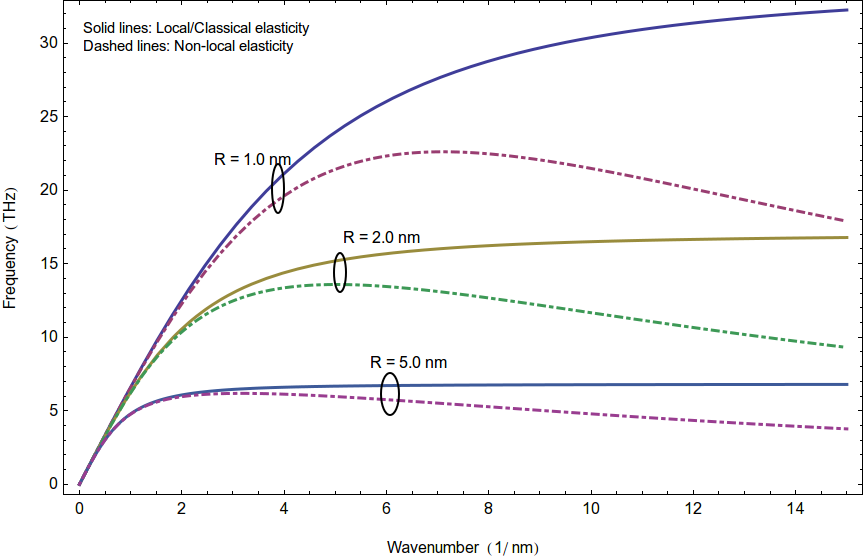
\includegraphics[scale=0.5]{varyradius.png}
\caption{Wavenumber dispersion (including the effect of lateral inertia) with wave
frequency in a nanorod obtained from both the local and nonlocal formulations for
different radii of nanorods.}
\label{varyradius}
\end{figure}

We have also analysed the behaviour of phase and group velocities using the models studied. This is illustrated in Fig. \ref{phasevel} and Fig. \ref{groupvel}. These plots also reinforce the observation that the strain gradient model (especially the second order strain gradient model) is not a stable model. Including lateral inertia in the stress gradient model indicates an improved response.

\begin{figure}
\centering
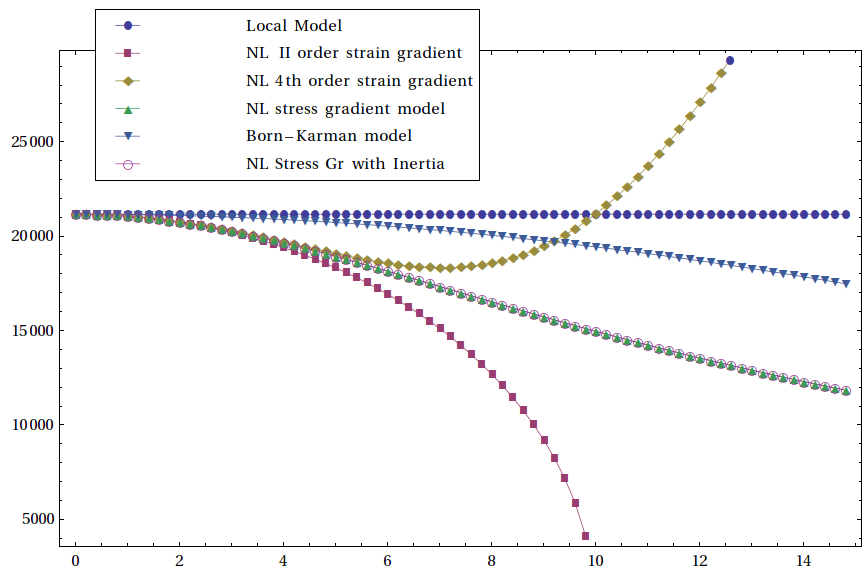
\includegraphics[scale=0.5]{phasevel.png}
\caption{Behaviour of phase velocity with varying wavenumber}
\label{phasevel}
\end{figure}

\begin{figure}
\centering
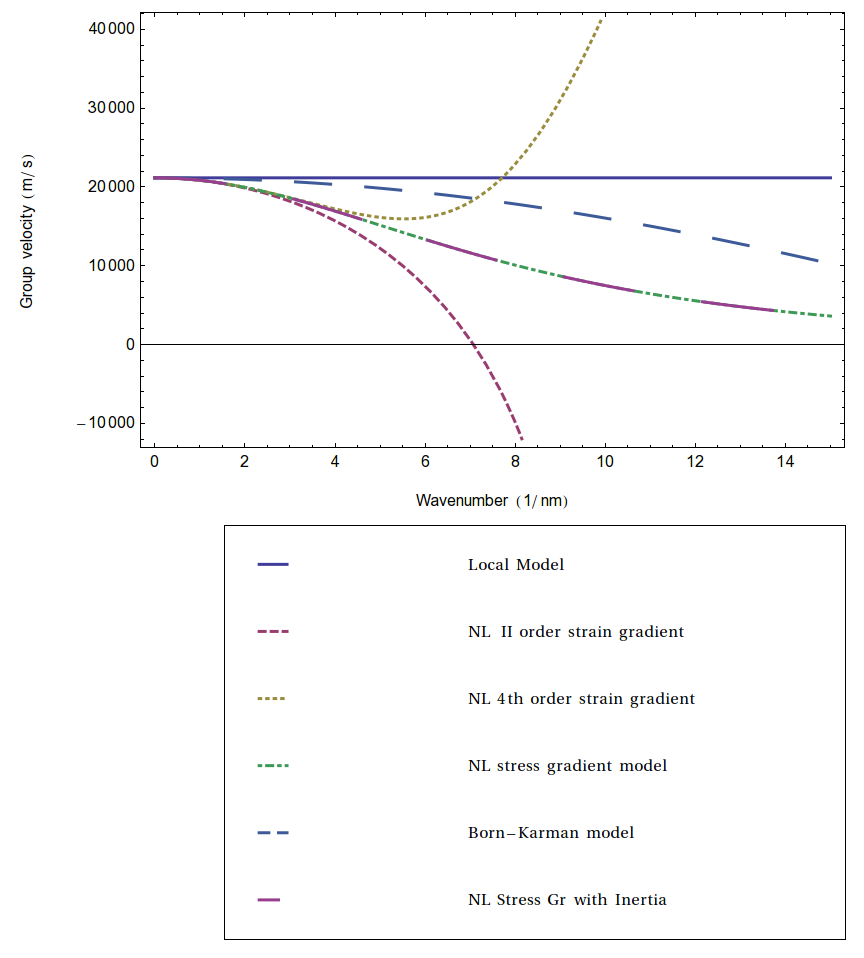
\includegraphics[scale=0.5]{groupvel.png}
\caption{Behaviour of group velocity with varying wavenumber}
\label{groupvel}
\end{figure}

\subsection{Conclusion}
It can be concluded that the wave dispersion characteristics in a
nanorod is drastically different for local and nonlocal models.
Where local model predicts that the wave will propagate at all
frequencies, but the nonlocal model shows that the wave will
propagate up to certain frequencies only depending on the nonlocal
scaling parameter. It has also been shown that, the unstable second
order strain gradient model can be replaced by considering the
inertia gradient terms in the formulations. 
